\chapter{Interfaţa aplicaţiei}
\label{chapter:interfata}

Aplicaţia dispune de o interfaţă modernă şi a fost implementată folosind standardul HTML5, cu pagini dinamice care păstrează starea în client, prin încărcarea asincrona a elementelor. Întreaga interfaţă este de tip responsive, scalându-se automat pentru afişare pe dispozitive cu rezoluţii diferite (monitor,  tabletă sau telefoane).

La accesarea aplicaţiei, utilizatorul este întâmpinat de interfaţă de autentificare din \cref{fig:login}. 
\begin{figure}[H]
	\centering
	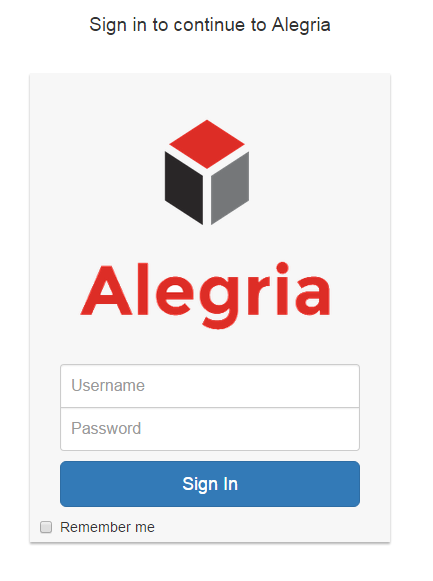
\includegraphics[width=0.5\textwidth]{screens/login}
	\captionsetup{justification=centering}
	\caption{Autentificarea în aplicaţie}
	\label{fig:login}
\end{figure}
Login-ul în aplicaţie permite accesul la interfaţa de management şi monitorizare. Navigaţia se face printr-un meniu aflat în antetul paginii, vizibil în \cref{fig:navMenu}
\begin{figure}[H]
	\centering
	
\includegraphics[width=\textwidth]{screens/navMenu}
	\captionsetup{justification=centering}
	\caption{Navigarea prin funcţiile aplicaţiei}
	\label{fig:navMenu}
\end{figure}
Dacă utilizatorul este administrator, atunci el poate accesa şi administrarea utilizatorilor. Aici el poate adăuga noi utilizatori, modifica utilizatorii existenţi sau poate dezactiva accesul unora din aplicaţie.
\begin{figure}[H]
	\centering
	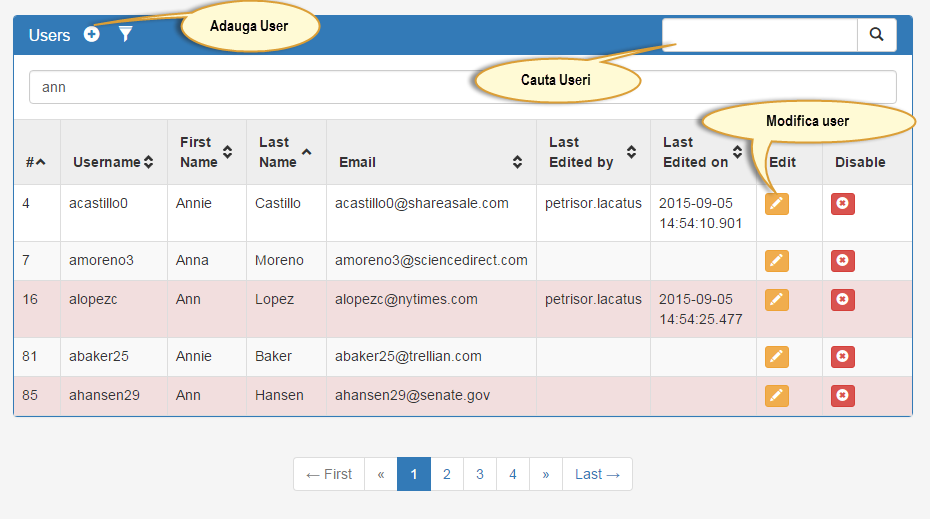
\includegraphics[width=1.2\textwidth, center]{screens/userManagement}
	\captionsetup{justification=centering}
	\caption{Managementul utilizatorilor din aplicaţie}
	\label{fig:userManagement}
\end{figure}
Toate entităţile dispun de o interfaţă similară cu cea din \cref{fig:userManagement}, în care utilizatorul are acces facil la entităţile existente în sistem. Tabelele în care datele sunt afişate permit sortarea şi filtrarea, uşurând astfel găsirea entităţii ce trebuie modificată. În plus, căutarea se poate face nu doar după numele entităţii, ci şi după taguri sau descriere. Conţinutul este paginat astfel încât timpul de încărcare a paginii să fie cât mai mic.

În cazul administrării blocurilor de intrare, un panou modal, încărcat dinamic, este disponibil pentru adăugare şi editare. În acest panou, utilizatorul poate seta taguri şi administra canalele de pe acel bloc.
\begin{figure}[H]
	\centering
	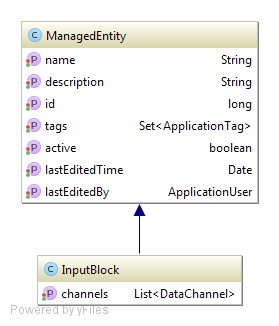
\includegraphics[width=\textwidth]{screens/inputBlock}
	\captionsetup{justification=centering}
	\caption{Editarea unui bloc de intrare}
	\label{fig:inputBlock}
\end{figure}

Pentru management-ul blocurile de procesare, utilizatorul are la dispoziţie şi un editor inteligent care afişează codul colorat în funcţie de limbajul selectat. Astfel, utilizatorii pot depista erorile de sintaxa în timpul editării codului.
\begin{figure}[H]
	\centering
	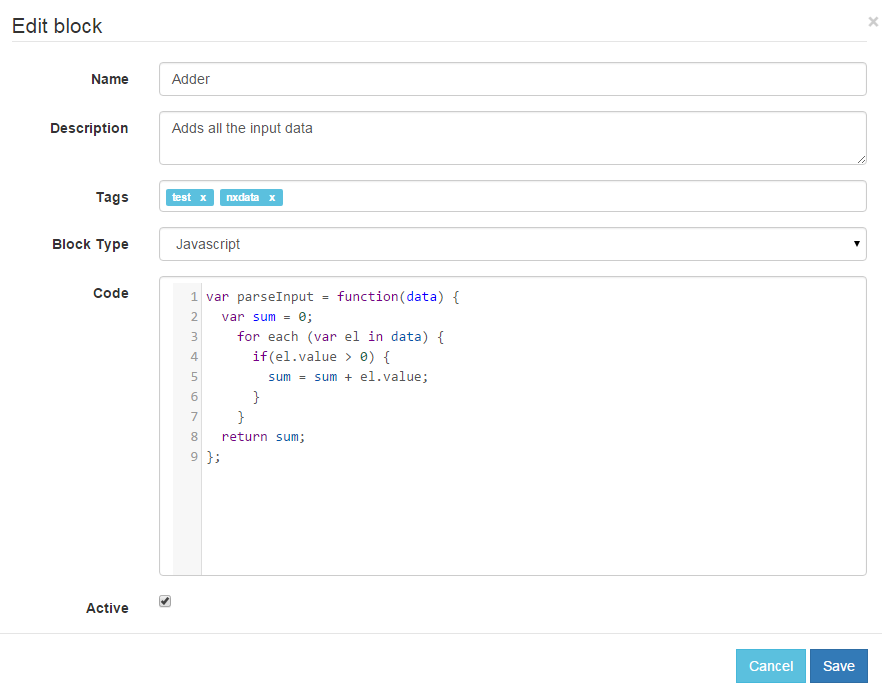
\includegraphics[width=1.1\textwidth, center]{screens/blockManagement}
	\captionsetup{justification=centering}
	\caption{Modificarea unui bloc de procesare şi editarea codului}
	\label{fig:blockManagement}
\end{figure}
Editarea diagramelor funcţionale se face vizual, într-o interfaţă asemănătoare cu cea din SimuLink sau LOGO! Soft Comfort. Aceasta interfaţă permite adăugarea vizuală a blocurilor dintr-o paletă, căutarea automată a instantelor de blocuri şi exportarea schemei diagramei pentru salvare într-un mediu extern. 

Blocurile pot fi modificate atât prin schimbarea proprietăţilor acestora din meniul ce apare în partea de jos a diagramei când blocul este selectat, dar şi direct prin acţiunea de click stânga sau dreapta pe acesta. Pentru blocurile de procesare, utilizatorul are opţiunea să vizualizeze şi să modifice codul direct din aceasta pagină, fără a mai naviga spre pagina de administrare a blocurilor de procesare.
Alături de câmpul de descriere, comentariile adăugate direct peste diagrama, ajută la documentarea implementării şi funcţionalităţii.
\begin{figure}[H]
	\centering
	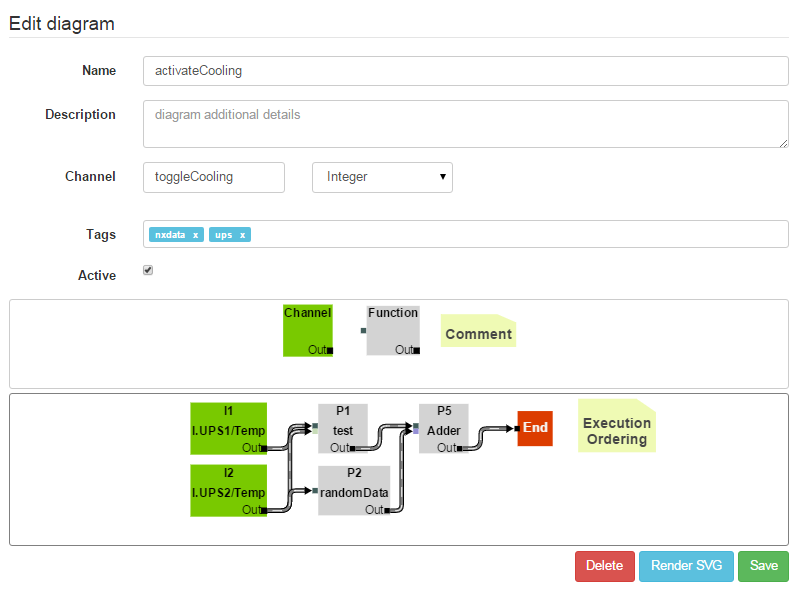
\includegraphics[width=1\textwidth, center]{screens/editDiagram}
	\captionsetup{justification=centering}
	\caption{Realizarea unei diagrame funcţionale}
	\label{fig:editDiagram}
\end{figure}

\begin{figure}[H]
	\centering
	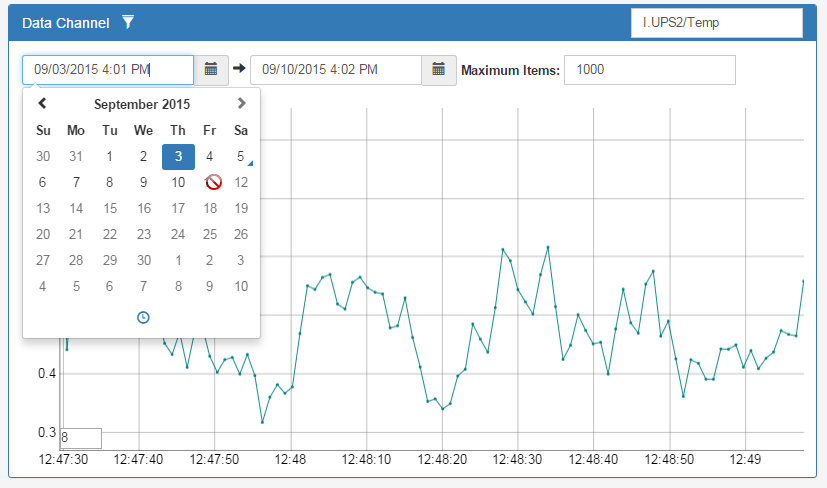
\includegraphics[width=1.1\textwidth, center]{screens/monitoring}
	\captionsetup{justification=centering}
	\caption{Monitorizarea datelor de pe un canal}
	\label{fig:monitoring}
\end{figure}